\begin{teamsubmission}{Parse Patrol}{Parse Patrol: Dual-Mode Scientific Parsing Infrastructure via MCP Servers}
\authorsblock{
    Nathan Daelman\textsuperscript{1}\orcidlink{0000-0002-7647-1816},
    Christina Ertural\textsuperscript{2}\orcidlink{0000-0002-7696-5824},
    Rubel Mozumber\textsuperscript{1}\orcidlink{0009-0007-5926-6646},
    Sascha Klawohn\textsuperscript{1}\orcidlink{0000-0003-4850-776X},
    Remya Ann Mathews Kalapurakal\textsuperscript{3} 
}
\affiliationsblock{
    \textsuperscript{1}Humboldt University of Berlin, 10117 Berlin, Germany\\
    \textsuperscript{2}Department of Materials Chemistry, Federal Institute for Materials Research and Testing, 12205 Berlin, Germany\\
    \textsuperscript{3}University of New Hampshire, 03824 Durham, NH, USA
}

\section*{Introduction}

Parsing scientific output files to extract structured data is by its very nature dependent on the input and output specifications.
These specifications may exist at a format level, a schema level, or more abstractly, an ontological one.
Being dependent on both sides, makes parser infrastructure very brittle and labor-intensive to maintain.

This is a frequent issue in (materials and chemistry) databases and consortia.
As they seek to structure these various schemas and formats into a more centralized standard, they risk breaking the output specifications of their parsers.
The community needs a robust procedure for rapidly rolling out updates at the standards and schemas side down to the infrastructure implementing them.
Furthermore, the uncoordinated approach of the community leaves individual projects vulnerable to funding or time cuts.\cite{}

Meanwhile, the rise of large language models (LLMs) has opened up new avenues for automating parser development.
Modern host environments, like IDEs, supply their LLM agents with testing, research, and other development tools.
Anthropic published the Model Context Protocol (MCP)\cite{mcp2024} late last year, defining a general-purpose, host-agnostic interface for such toolkits.
It has since rapidly become the industry standard and is now supported by all major commercial models.
MCP defines a schema in JSON-RPC 2.0 format for communication between agents and a server that exposes several \textit{components}: software \textit{tools}, static and dynamic \textit{resources}, and specially designed system \textit{prompts}.

In this work, we present Parse Patrol, an extensible parsing toolkit for AI and human developers alike.
Parse Patrol takes advantage of MCP to integrate various community parsers into a single access point.
It facilitates both (i) a discovery mode, where an agent test the various parsers out for converting to a user-defined schema,
as well as a (ii) direct import mode, where the parsers can be called as modules from code.

\section*{Results}

Parse Patrol starts from observing automated parser scripting and the various pitfalls that may arise.
The lack of online resources for scientific specifications will impede any on-the-fly research.
A developer will now have to turn to Retrieval-Augmented Generation and build out their own knowledgebase first.
When a request falls outside its scope, the model is still liable to hallucinate answers.
Even with the appropriate context, agents often require long test iteration cycles before settling on a working prototype.
Finally, agents are prone to radically overhauling the software architecture.

To circumvent these hurdles we turn to specialized community parsers.
Their inclusion enables fast, high-fidelity data extraction and reliable format conversion
We provide direct access to these parsers and their documentation via the MCP tools and resources, respectively.
This allows the project developers to focus on building out a wide coverage.
Not only does this cover more specifications, but it also introduces multiple synergetic design options.

Note that MCP does not provide any directives on how to extend the layer in a structured fashion: by default, one just extends the list of tools.
Our first technical innovation is thus to define a hierarchical protocol for extending the MCP server.
Each parser is treated as its own MCP server.
This facilitates testing, as the developer can instantiate just that single server.
All MCP components are then automatically registered to the central, user-facing server.
This server predominantly adds its own engineered prompts for deploying tests or production.
Specifications are provided directly in the chat or as a separate file.
Test cases can be downloaded via database MCP servers.
At the time of writing, Parse Patrol only supports downloads from NOMAD-lab\cite{nomad_lab,draxl2019nomad}.

Where the MCP empowers interactive testing and development, actual parsing infrastructure requires code in production.
We observed ourselves that even with access to an MCP parsing server, the agent will -- without explicit prompting -- revert back to generating domain-specific parsers from first principles.
Doing so, it may fall back on to its training or online research how 
Alternatively, it may attempt to find the installation path of the MCP server code itself and use it as a template.

Therefore, we provide the MCP tools, normally reserved for the discovery phase, as code modules too.
As modules, we also guarantee their installation setup, further offloading a burden of the agent.

Even so, the agent will not automatically pick up on these modules.
We attribute this behavior to the underlying models not having been trained on a MCP/module hybrid.
Our solution is two-pronged: we provide instructions in the relevant prompts to use the modules.
Each parser server exposes its module path and how to call it as a resource.
These are then compiled into a list of resources at the central server detailed above.

Providing such a common solution that is both a MCP sever and a module is not easy.
Each framework has different requirements and is distributed via different channels: \href{https://github.com/modelcontextprotocol/servers}{MCP Registry}\cite{mcp2024registry} and \href{https://pypi.org/}{PyPi}\cite{pypi}, respectively, for example.
Our second innovation, then, is the design of a \textit{dual mode} (cf. Fig.\ref{fig:parse-patrol}) that facilitates the free combination of either feature.
To the best of the authors' knowledge, no other such framework exists that bridges the divide between AI experimentation and production integration.

\begin{figure}[h]
    \centering
    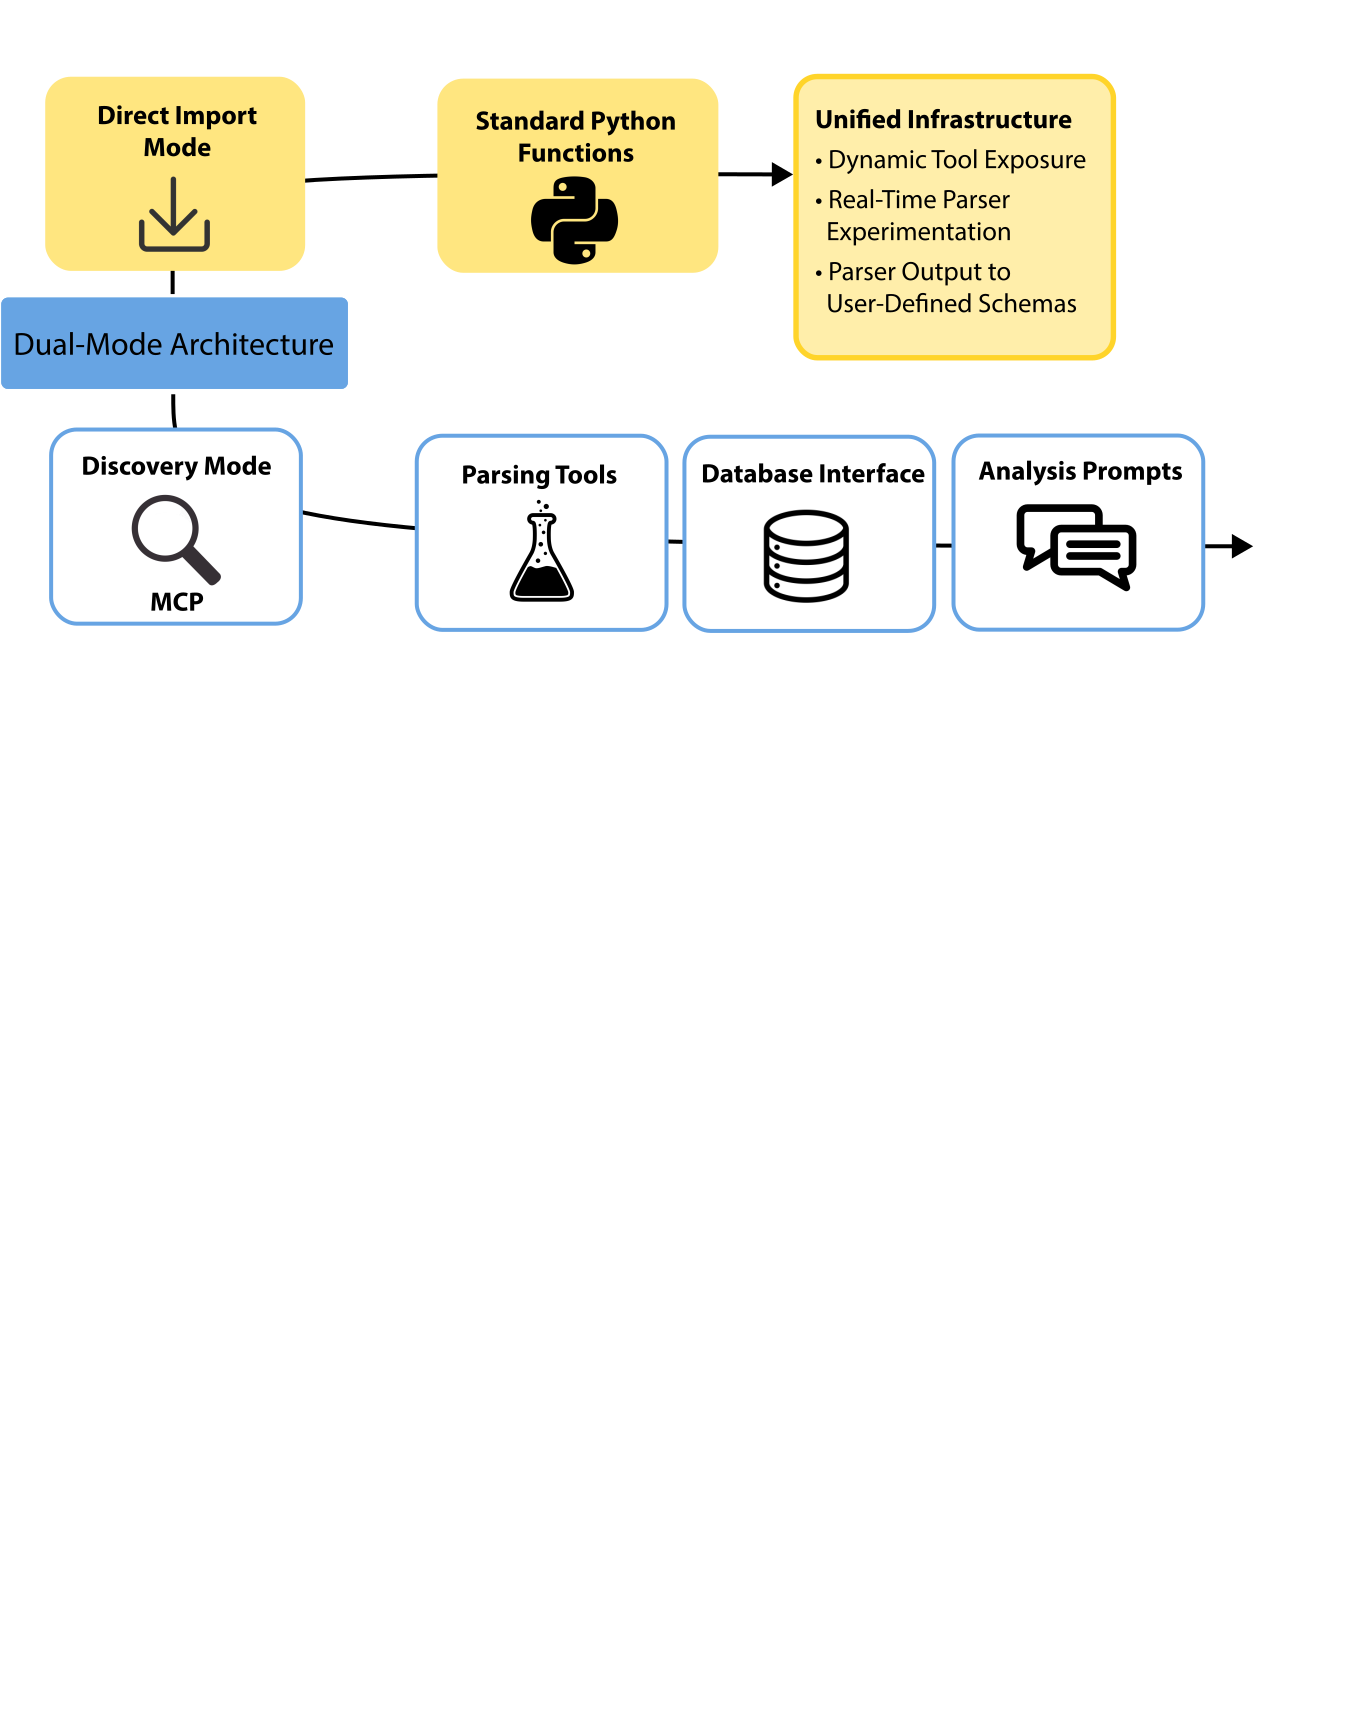
\includegraphics[width=0.5\linewidth]{figures/parse-patrol.png}
    \caption{
    \textbf{Parse Patrol:}
    Schematic depiction of the \textit{dual-mode} design.
    Lower branch: Discovery mode provides a single MCP interface to several parser and database servers.
    The central server further exposes pre-engineered prompts for the suggested use case.
    Most hosts provide shortcuts to these prompts.
    Upper branch: Direct Import mode exposes the same MCP components as Python modules for friction-less switching from testing to production.
    Both branches are unified under a unified architecture.
    }
    \label{fig:parse-patrol}
\end{figure}

\section*{Future Work}

At the time of writing, the repository is seeing active development.
Recent additions include automated registration of all the subservers.
Given the well-defined objective of providing a computational parsers toolkit, future extensions are not excluded.
This project is under consideration for incorporation into NOMAD parser suite.

\section*{Open Source Materials}

The open source code is available on GitHub: \github{https://github.com/ndaelman-hu/parse-patrol}. 
A demo video is available on YouTube: \youtube{https://www.youtube.com/watch?v=fSAyi5ubkR0}.

\section*{Author Contributions}

\textbf{N.D.}: Conceptualization, Software, Original Code Draft, Visualization, Writing - Editing
\textbf{C.E.}: Conceptualization Revision, Software, Visualization, Video Editing, Writing - Original Manuscript Text Draft, Figure, Editing
\textbf{R.M.}: Implementation asynchronous servers, Extension Testing Infrastructure - Conceptualization Revision
\textbf{S.K.}: Extend Parser Servers - Proof-read Submission

\section*{Acknowledgements}
This work was supported by the NFDI consortium FAIRmat - Deutsche Forschungsgemeinschaft (DFG) - Project 460197019.

\end{teamsubmission}